\part{Contributions et Implementation}
\chapter{Endormissement de tache sous priorité Fixe}
\minitoc
\section{modéle de tâches}
\indent Le modèle utilisé ici est le modèle de tâche périodique de Liu et Layland défini au chapitre 1.\\
Soit $\taskset = \{\tache{1},\tache{2},...,\tache{n}\}$ un ensemble de tache, chaque tache $\tache{i}$ est caracterisé par $\tache{i} = (\wcet{i},\deadline{i},\periode{i})$ et :
\begin{itemize}
\item[$\bullet$] $\tache{i}$ est periodique.
\item[$\bullet$] $\wcet{i}$ est le pire temps d'execution de la tache$_i$.
\item[$\bullet$] $\deadline{i}$ est l'écheance relative de la tache$_i$.
\item[$\bullet$] $\periode{i}$ est la periode relative de la tache$_i$.
\item[$\bullet$] l'ensemble de tâches $\taskset$ est ordonnançable avec l'algorithme Deadline Monotonic.
\end{itemize}
\section{Le cas monoprocesseur}
\indent Dans cette section nous allons inserer une tâche d'endormissement $\tache{sleep} = \{ \wcet{sleep}, \deadline{sleep}, \periode{sleep}\}$
avec $\wcet{sleepMin} \leq \wcet{sleep} \geq \wcet{sleepMax}$ avec $\wcet{sleepMax} = (1-\util{}) \times \periode{H}$ et $\tache{sleep} \cup \taskset$ est ordonnançable avec Deadline Monotonic. \\
\indent Pour cela nous presentons l'algorithme d'insertion de tache d'endormissement $\tache{sleep}$ dans un taskset $\taskset$.
\begin{center}
\begin{algorithm}[H]
\KwData{TaskSet $\taskset{}$, Temps Minimum d'execution $\wcet{SleepMin}$, Temps d'execution Maximum $\wcet{SleepMax}$, Pas de decrementation $\Delta \wcet{}$}
\KwResult{Tache $\tache{Sleep}$}
\Begin{
 $\wcet{Sleep}  \longleftarrow \wcet{SleepMax}$ \;
 $\deadline{Sleep}	\longleftarrow \periode{H}$ \;
 $\periode{sleep} \longleftarrow \periode{H}$ \;
 \While{$\Gamma \cup tache(\wcet{Sleep},\deadline{Sleep},\periode{H})$ est non  ordonnançable et $\wcet{Sleep} \geq \wcet{SleepMin}$}
 {
 	$\wcet{Sleep} \longleftarrow \wcet{Sleep} - \Delta \wcet{}$ \;
 }
 $\tache{Sleep} \longleftarrow CreerTache(\wcet{Sleep},\deadline{Sleep},\periode{sleep})$
 }
 \caption{Insertion Taches Endormissement Dans Un Mono-processeur}
\end{algorithm}
\end{center} 
\indent Nous illustrons notre algorithme avec un exemple d'application. Le tableau \ref{tab:exempledmup} et la figure \ref{fig:exempledmupapr} represente un ensemble de tâches $\taskset$ 
ordonnançable par Deadline Monotonic où on a inseré une tache d'endormissement $\tache{sleep}$

\begin{table}[!h]
\begin{center}
\begin{tabular}{|c|c|c|c|}
 \hline$\tache{i}$ & $\wcet{i}$ & $\deadline{i}$ & $\periode{i}$ \\ 
 \hline 1 & 1 & 10 & 10 \\ 
 \hline 2 & 2 & 15 & 15 \\ 
 \hline 
 \end{tabular}
\end{center}
\caption{Ensemble de taches periodiques} \label{tab:exempledmup}
\end{table}

\begin{figure}[h]
\begin{center}
\begin{RTGrid}[height=4cm,width=12cm,labelsize=8pt,numbersize=6]{3}{31}
\multido{\n=0+10}{3}{
\TaskArrDead{1}{\n}{10}}
\TaskArrDead{1}{20}{10}

\TaskExecution{1}{3}{4}
\TaskExecution{1}{13}{14}
\TaskExecution{1}{23}{24}

\multido{\n=0+15}{2}{
\TaskArrDead{2}{\n}{15}}
\TaskArrDead{2}{15}{15}
\TaskExecution{2}{4}{5}
\TaskExecution{2}{8}{9}
\TaskExecution{2}{18}{20}

\multido{\n=0+5}{6}{
\TaskArrDead{3}{\n}{5}}
\TaskArrDead{3}{25}{5}
\TaskExecution{3}{0}{3}
\TaskExecution{3}{5}{8}
\TaskExecution{3}{10}{13}
\TaskExecution{3}{15}{18}
\TaskExecution{3}{20}{23}
\TaskExecution{3}{25}{28}

\end{RTGrid}
\caption{Insertion de tache dans un monoprocesseur} \label{fig:exempledmup}
\end{center}
\end{figure}

\section{Le cas multiprocesseur}
\indent Dans cette section nous allons inserer un ensemble de tâches d'endormissement $\{\tache{sleep}^1,\tache{sleep}^2,...,\tache{sleep}^m\}$ tel que $\tache{sleep}^i = \{ \wcet{sleep}^i, \deadline{sleep}^i, \periode{sleep}^i\}$
dans m processeurs $\proc{} = \{\proc{1},\proc{2},...,\proc{m}\}$.
\indent Pour cela nous presentons nous presentons deux strategie d'insertion :
\begin{description}
\item{Insertion Locale :} Chaque processeur$_i$ à sa propre tache d'endormissement $\tache{sleep}^i$
\item{Insertion Globale :} Tous les processeur ont une même tache d'endormissement $\tache{sleep}=\tache{sleep}^1=\tache{sleep}^2=...=\tache{sleep}^m$
\end{description}
\indent Les deux algorithmes representent l'inseretion locale (Resp. globale) d'un ensemble de tâches d'endormissement dans un ensemble de processeur.
\begin{center}
\begin{algorithm}[H]
\KwData{Ensemble de processeur $\proc{}$, Temps Minimum d'execution $\wcet{SleepMin}$}
\KwResult{Ensemble de Tache d'endormissement $\taskset{Sleep}$}
\Begin{
	\For{$ \proc{i} \in \proc{}$}
	{
		$\tache{sleep}^i$ = tache\_endormissement\_monoprocesseur($\wcet{SleepMin}$) \; 
		$\taskset{Sleep}^i =\taskset{Sleep}^i \cup \tache{sleep}^i$
		}
	}
 \caption{Insertion Globale de Taches Endormissement Dans Une architecture Multiprocesseur}
\end{algorithm}
\end{center} 
\begin{center}
\begin{algorithm}[H]
\KwData{Ensemble de processeur $\proc{}$, Temps Minimum d'execution $\wcet{SleepMin}$}
\KwResult{Ensemble de Tache d'endormissement $\taskset{Sleep}$}
\Begin{
	$\tache{sleep} \rightarrow \emptyset$ \;
	\For{$ \proc{i} \in \proc{}$}
	{
		$\tache{sleep}^i$ = tache\_endormissement\_monoprocesseur($\wcet{SleepMin}$) \; 
		$\tache{sleep} \rightarrow \tache{sleep} \cup \tache{sleep}^i$
	}
	\For{$ \proc{i} \in \proc{}$}
	{
		$\taskset{sleep}^i \rightarrow \taskset{sleep}^i \cup Min_{i =1..m}(\tache{sleep}^i)$
	}
	}
 \caption{Insertion Globale de Taches Endormissement Dans Une architecture Multiprocesseur}
\end{algorithm}
\end{center} 
\indent Nous illustrons notre algorithme avec un exemple d'application. Le tableau \ref{tab:exempledmmp} et les figures \ref{fig:exempledmmpl} et \ref{fig:exempledmmpg} representent un ensemble de tâches $\taskset$ 
ordonnançable par Deadline Monotonic dans un multiprocesseur à 2 processeur en partitionnement FirstFit où on a inseré deux taches d'endormissements $\tache{sleep}$ en locale et en globale.
\begin{table}[!h]
\begin{center}
\begin{tabular}{|c|c|c|c|}
 \hline$\tau_i$ & $C_i$ & $D_i$ & $T_i$ \\ 
 \hline1 & 5 & 10 & 10 \\ 
 \hline 2 & 7 & 15 & 21 \\ 
 \hline 3 & 2 & 22 & 24 \\ 
 \hline 
 \end{tabular}
\end{center}
\caption{Ensemble de tâche périodique} \label{tab:dmmp}
\end{table}
\begin{figure}[!h]
\begin{center}
\resizebox{15cm}{4cm}{
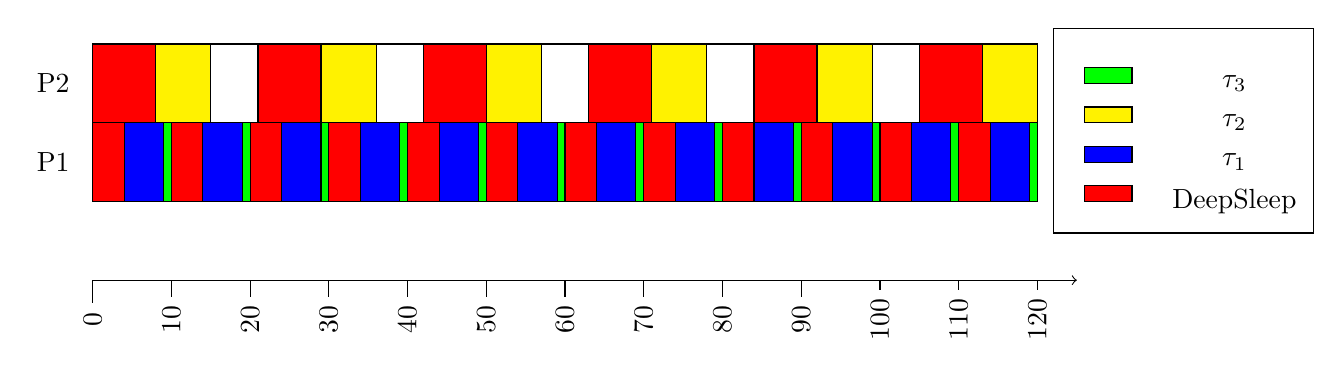
\begin{tikzpicture}
\node at (-0.5,0.5) {P1};
\node at (-0.5,1.5) {P2};
%P1 DS
\draw[fill=red] (0,0) rectangle (0.4,1) ;
\draw[fill=red] (1,0) rectangle (1.4,1) ;
\draw[fill=red] (2,0) rectangle (2.4,1) ;
\draw[fill=red] (3,0) rectangle (3.4,1) ;
\draw[fill=red] (4,0) rectangle (4.4,1) ;
\draw[fill=red] (5,0) rectangle (5.4,1) ;
\draw[fill=red] (6,0) rectangle (6.4,1) ;
\draw[fill=red] (7,0) rectangle (7.4,1) ;
\draw[fill=red] (8,0) rectangle (8.4,1) ;
\draw[fill=red] (9,0) rectangle (9.4,1) ;
\draw[fill=red] (10,0) rectangle (10.4,1) ;
\draw[fill=red] (11,0) rectangle (11.4,1) ;
%P1 T1
\draw[fill=blue] (0.4,0) rectangle (0.9,1) ;
\draw[fill=blue] (1.4,0) rectangle (1.9,1) ;
\draw[fill=blue] (2.4,0) rectangle (2.9,1) ;
\draw[fill=blue] (3.4,0) rectangle (3.9,1) ;
\draw[fill=blue] (4.4,0) rectangle (4.9,1) ;
\draw[fill=blue] (5.4,0) rectangle (5.9,1) ;
\draw[fill=blue] (6.4,0) rectangle (6.9,1) ;
\draw[fill=blue] (7.4,0) rectangle (7.9,1) ;
\draw[fill=blue] (8.4,0) rectangle (8.9,1) ;
\draw[fill=blue] (9.4,0) rectangle (9.9,1) ;
\draw[fill=blue] (10.4,0) rectangle (10.9,1) ;
\draw[fill=blue] (11.4,0) rectangle (11.9,1) ;
%P1 T3
\draw[fill=green] (0.9,0) rectangle (1,1) ;
\draw[fill=green] (1.9,0) rectangle (2,1) ;
\draw[fill=green] (2.9,0) rectangle (3,1) ;
\draw[fill=green] (3.9,0) rectangle (4,1) ;
\draw[fill=green] (4.9,0) rectangle (5,1) ;
\draw[fill=green] (5.9,0) rectangle (6,1) ;
\draw[fill=green] (6.9,0) rectangle (7,1) ;
\draw[fill=green] (7.9,0) rectangle (8,1) ;
\draw[fill=green] (8.9,0) rectangle (9,1) ;
\draw[fill=green] (9.9,0) rectangle (10,1) ;
\draw[fill=green] (10.9,0) rectangle (11,1) ;
\draw[fill=green] (11.9,0) rectangle (12,1) ;

\draw[fill=red] (0.0,1) rectangle (0.8,2) ;
\draw[fill=yellow] (0.8,1) rectangle (1.5,2) ;
\draw[fill=white] (1.5,1) rectangle (2.1,2) ;

\draw[fill=red] (2.1,1) rectangle (2.899999904632568,2) ;
\draw[fill=yellow] (2.899999904632568,1) rectangle (3.5999999046325684,2) ;
\draw[fill=white] (3.5999999046325684,1) rectangle (4.199999904632568,2) ;

\draw[fill=red] (4.2,1) rectangle (4.9999998092651365,2) ;
\draw[fill=yellow] (4.9999998092651365,1) rectangle (5.699999809265137,2) ;
\draw[fill=white] (5.699999809265137,1) rectangle (6.299999809265136,2) ;

\draw[fill=red] (6.2999997,1) rectangle (7.099999713897705,2) ;
\draw[fill=yellow] (7.099999713897705,1) rectangle (7.799999713897705,2) ;
\draw[fill=white] (7.799999713897705,1) rectangle (8.399999713897705,2) ;

\draw[fill=red] (8.4,1) rectangle (9.199999618530274,2) ;
\draw[fill=yellow] (9.199999618530274,1) rectangle (9.899999618530273,2) ;
\draw[fill=white] (9.899999618530273,1) rectangle (10.499999618530273,2) ;

\draw[fill=red] (10.5,1) rectangle (11.3,2) ;
\draw[fill=yellow] (11.3,1) rectangle (12.0,2) ;

\draw [->](0,-1) -- coordinate (x axis mid) (12.5,-1);
\draw (0,-1) -- (0,-1.5) node[fill=white,rotate=90] {0};
\draw (1,-1) -- (1,-1.5) node[fill=white,rotate=90] {10};
\draw (2,-1) -- (2,-1.5) node[fill=white,rotate=90] {20};
\draw (3,-1) -- (3,-1.5) node[fill=white,rotate=90] {30};
\draw (4,-1) -- (4,-1.5) node[fill=white,rotate=90] {40};
\draw (5,-1) -- (5,-1.5) node[fill=white,rotate=90] {50};
\draw (6,-1) -- (6,-1.5) node[fill=white,rotate=90] {60};
\draw (7,-1) -- (7,-1.5) node[fill=white,rotate=90] {70};
\draw (8,-1) -- (8,-1.5) node[fill=white,rotate=90] {80};
\draw (9,-1) -- (9,-1.5) node[fill=white,rotate=90] {90};
\draw (10,-1) -- (10,-1.5) node[fill=white,rotate=90] {100};
\draw (11,-1) -- (11,-1.5) node[fill=white,rotate=90] {110};
\draw (12,-1) -- (12,-1.5) node[fill=white,rotate=90] {120};

\draw[fill=white] (12.2,-0.4) rectangle (15.5,2.2) ;
\draw[fill=red] (12.6,0) rectangle (13.2,0.2) ;
\draw (14.5,0) -- (14.5,0) node[fill=white] {DeepSleep};
\draw[fill=blue] (12.6,0.5) rectangle (13.2,0.7) ;
\draw (14.5,0.5) -- (14.5,0.5) node[fill=white] {$\tau_1$};
\draw[fill=yellow] (12.6,1) rectangle (13.2,1.2) ;
\draw (14.5,1) -- (14.5,1) node[fill=white] {$\tau_2$};
\draw[fill=green] (12.6,1.5) rectangle (13.2,1.7) ;
\draw (14.5,1.5) -- (14.5,1.5) node[fill=white] {$\tau_3$};
\end{tikzpicture}}
\end{center}
\caption{Insertion locale de tâches d'endormissements dans un multiprocesseur} \label{fig:dmmpl}
\end{figure}
\begin{figure}[!h]
\begin{center}
\resizebox{15cm}{4cm}{
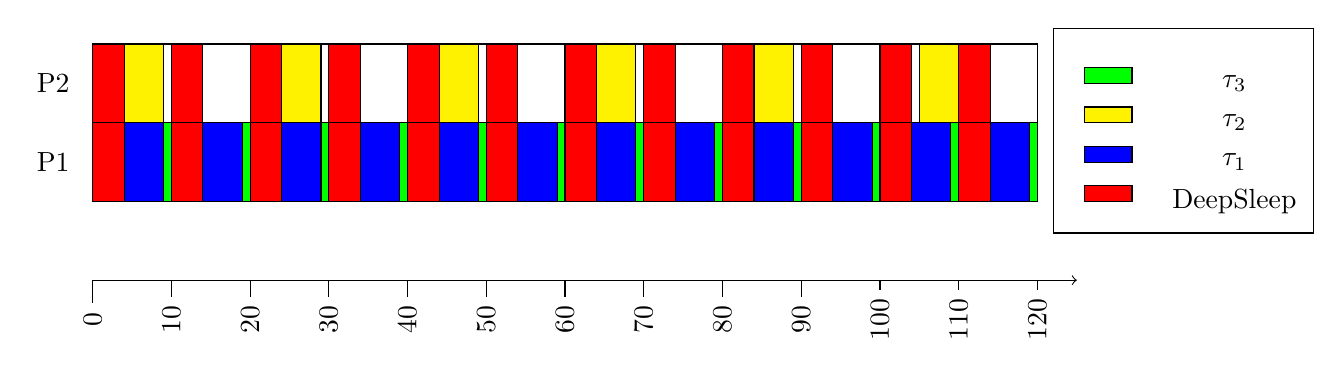
\begin{tikzpicture}
\node at (-0.5,0.5) {P1};
\node at (-0.5,1.5) {P2};
%P1 DS
\draw[fill=red] (0,0) rectangle (0.4,1) ;
\draw[fill=red] (1,0) rectangle (1.4,1) ;
\draw[fill=red] (2,0) rectangle (2.4,1) ;
\draw[fill=red] (3,0) rectangle (3.4,1) ;
\draw[fill=red] (4,0) rectangle (4.4,1) ;
\draw[fill=red] (5,0) rectangle (5.4,1) ;
\draw[fill=red] (6,0) rectangle (6.4,1) ;
\draw[fill=red] (7,0) rectangle (7.4,1) ;
\draw[fill=red] (8,0) rectangle (8.4,1) ;
\draw[fill=red] (9,0) rectangle (9.4,1) ;
\draw[fill=red] (10,0) rectangle (10.4,1) ;
\draw[fill=red] (11,0) rectangle (11.4,1) ;
%P1 T1
\draw[fill=blue] (0.4,0) rectangle (0.9,1) ;
\draw[fill=blue] (1.4,0) rectangle (1.9,1) ;
\draw[fill=blue] (2.4,0) rectangle (2.9,1) ;
\draw[fill=blue] (3.4,0) rectangle (3.9,1) ;
\draw[fill=blue] (4.4,0) rectangle (4.9,1) ;
\draw[fill=blue] (5.4,0) rectangle (5.9,1) ;
\draw[fill=blue] (6.4,0) rectangle (6.9,1) ;
\draw[fill=blue] (7.4,0) rectangle (7.9,1) ;
\draw[fill=blue] (8.4,0) rectangle (8.9,1) ;
\draw[fill=blue] (9.4,0) rectangle (9.9,1) ;
\draw[fill=blue] (10.4,0) rectangle (10.9,1) ;
\draw[fill=blue] (11.4,0) rectangle (11.9,1) ;
%P1 T3
\draw[fill=green] (0.9,0) rectangle (1,1) ;
\draw[fill=green] (1.9,0) rectangle (2,1) ;
\draw[fill=green] (2.9,0) rectangle (3,1) ;
\draw[fill=green] (3.9,0) rectangle (4,1) ;
\draw[fill=green] (4.9,0) rectangle (5,1) ;
\draw[fill=green] (5.9,0) rectangle (6,1) ;
\draw[fill=green] (6.9,0) rectangle (7,1) ;
\draw[fill=green] (7.9,0) rectangle (8,1) ;
\draw[fill=green] (8.9,0) rectangle (9,1) ;
\draw[fill=green] (9.9,0) rectangle (10,1) ;
\draw[fill=green] (10.9,0) rectangle (11,1) ;
\draw[fill=green] (11.9,0) rectangle (12,1) ;

\draw[fill=white] (0,1) rectangle (12,2) ;
\draw[fill=red] (0,1) rectangle (0.4,2) ;
\draw[fill=red] (1,1) rectangle (1.4,2) ;
\draw[fill=red] (2,1) rectangle (2.4,2) ;
\draw[fill=red] (3,1) rectangle (3.4,2) ;
\draw[fill=red] (4,1) rectangle (4.4,2) ;
\draw[fill=red] (5,1) rectangle (5.4,2) ;
\draw[fill=red] (6,1) rectangle (6.4,2) ;
\draw[fill=red] (7,1) rectangle (7.4,2) ;
\draw[fill=red] (8,1) rectangle (8.4,2) ;
\draw[fill=red] (9,1) rectangle (9.4,2) ;
\draw[fill=red] (10,1) rectangle (10.4,2) ;
\draw[fill=red] (11,1) rectangle (11.4,2) ;

\draw[fill=yellow] (0.4,1) rectangle (0.9,2) ;
\draw[fill=yellow] (2.4,1) rectangle (2.9,2) ;
\draw[fill=yellow] (4.4,1) rectangle (4.9,2) ;
\draw[fill=yellow] (6.4,1) rectangle (6.9,2) ;
\draw[fill=yellow] (8.4,1) rectangle (8.9,2) ;
\draw[fill=yellow] (10.5,1) rectangle (11,2) ;

\draw [->](0,-1) -- coordinate (x axis mid) (12.5,-1);
\draw (0,-1) -- (0,-1.5) node[fill=white,rotate=90] {0};
\draw (1,-1) -- (1,-1.5) node[fill=white,rotate=90] {10};
\draw (2,-1) -- (2,-1.5) node[fill=white,rotate=90] {20};
\draw (3,-1) -- (3,-1.5) node[fill=white,rotate=90] {30};
\draw (4,-1) -- (4,-1.5) node[fill=white,rotate=90] {40};
\draw (5,-1) -- (5,-1.5) node[fill=white,rotate=90] {50};
\draw (6,-1) -- (6,-1.5) node[fill=white,rotate=90] {60};
\draw (7,-1) -- (7,-1.5) node[fill=white,rotate=90] {70};
\draw (8,-1) -- (8,-1.5) node[fill=white,rotate=90] {80};
\draw (9,-1) -- (9,-1.5) node[fill=white,rotate=90] {90};
\draw (10,-1) -- (10,-1.5) node[fill=white,rotate=90] {100};
\draw (11,-1) -- (11,-1.5) node[fill=white,rotate=90] {110};
\draw (12,-1) -- (12,-1.5) node[fill=white,rotate=90] {120};

\draw[fill=white] (12.2,-0.4) rectangle (15.5,2.2) ;
\draw[fill=red] (12.6,0) rectangle (13.2,0.2) ;
\draw (14.5,0) -- (14.5,0) node[fill=white] {DeepSleep};
\draw[fill=blue] (12.6,0.5) rectangle (13.2,0.7) ;
\draw (14.5,0.5) -- (14.5,0.5) node[fill=white] {$\tau_1$};
\draw[fill=yellow] (12.6,1) rectangle (13.2,1.2) ;
\draw (14.5,1) -- (14.5,1) node[fill=white] {$\tau_2$};
\draw[fill=green] (12.6,1.5) rectangle (13.2,1.7) ;
\draw (14.5,1.5) -- (14.5,1.5) node[fill=white] {$\tau_3$};
\end{tikzpicture}}
\end{center}
\caption{Insertion globale de tâches d'endormissements dans un multiprocesseur} \label{fig:dmmpg}
\end{figure}
\chapter{Endormissement de tache sous priorité dynamique}
\minitoc
\section{modéle de tâches}
\indent Le modèle utilisé ici est le modèle de tâche sporadique.\\
Soit $\taskset = \{\tache{1},\tache{2},...,\tache{n}\}$ un ensemble de tache, chaque tache $\tache{i}$ est caracterisé par $\tache{i} = (\wcet{i},\deadline{i},\periode{i})$ et :
\begin{itemize}
\item[$\bullet$] $\tache{i}$ est sporadique.
\item[$\bullet$] $\wcet{i}$ est le pire temps d'execution de la tache$_i$
\item[$\bullet$] $\deadline{i}$ est l'écheance relative de la tache$_i$
\item[$\bullet$] $\periode{i}$ est la periode de la tache$_i$
\item[$\bullet$] l'ensemble de tâches $\taskset$ est ordonnançable avec l'algorithme EarliestDeadlineFirst
\end{itemize}
\section{Limitation de nombre de preemption}
\begin{center}
\begin{algorithm}[H]
\KwData{TaskSet de tâches sporadic $\taskset{}$}
\KwResult{$Q(t)$}
\Begin{
 Posons $\{t_{1},t_{2},...,t_{n}\}$ ensemble ordonné de $\{\deadline{i}+l\periode{i},\forall l \in N, 1 \leq i \leq n \}$ où $(t_{k} < t_{k+1},\forall k)$
 $Q(t_{1}) \leftarrow t_{1} - \sum_{\tache{i} \in \taskset{}} DBF(\tache{i},t_{1})$\;
 \For{$k \leftarrow 2,3...$}{
	$Q(t_{k}) \leftarrow Min(Q(t_{k-1}),t_{k} - \sum_{\tache{i} \in \taskset{}} DBF(\tache{i},t_{k}))$\;
	\If{$Q(t_{k}) < 0$}{
	\textbf{return} faux\;
	}
	}
	\textbf{return} vrai\;
 }
 \caption{Insertion Taches Endormissement Dans Un Mono-processeur}
\end{algorithm}
\end{center} 
\section{Le cas monoprocesseur}
%\begin{center}
\begin{algorithm}[H]
\KwData{TaskSet $\taskset{}$, Temps Minimum d'execution $\wcet{SleepMin}$, Temps d'execution Maximum $\wcet{SleepMax}$, Pas de decrementation $\Delta \wcet{}$}
\KwResult{Tache $\tache{Sleep}(\wcet{Sleep},\deadline{Sleep},\periode{sleep})$}
\Begin{
 $\wcet{Sleep}  \longleftarrow \wcet{SleepMax}$ \;
 $\deadline{Sleep}	\longleftarrow \periode{H}$ \;
 $\periode{sleep} \longleftarrow \periode{H}$ \;
 
 \Repeat{$\Gamma \cup \tache{sleep}$ est non  ordonnançable et $\wcet{Sleep} > \wcet{SleepMin}$ et !test(\tache{sleep})}
 {
    calcule($\Gamma \cup \tache{sleep}$) \;
 	$\wcet{Sleep} \longleftarrow \wcet{Sleep} - \Delta \wcet{}$ \;
 }
 \eIf{$\Gamma \cup \tache{sleep}$ est non ordonnançable ou $\wcet{Sleep} \leq \wcet{SleepMin}$ ou !test(\tache{sleep})}{
    $\wcet{Sleep}  \longleftarrow 0$
    }
 }
 \caption{Insertion Taches Endormissement Dans Un Mono-processeur}
\end{algorithm}
\end{center}


\begin{table}[!h]
\begin{center}
\begin{tabular}{|c|c|c|c|}
 \hline$\tache{i}$ & $\wcet{i}$ & $\deadline{i}$ & $\periode{i}$ \\ 
 \hline 1 & 2 & 25 & 25 \\ 
 \hline 2 & 2 & 10 & 10 \\ 
 \hline 
 \end{tabular}
\end{center}
\caption{Ensemble de taches periodiques} \label{tab:exempleedfmp}
\end{table}

\begin{figure}[h]
\begin{center}
\begin{RTGrid}[height=4cm,width=12cm,labelsize=8pt,numbersize=6]{3}{32}

\multido{\n=0+25}{1}{
\TaskArrDead{1}{\n}{25}}
%\TaskArrDead{1}{20}{10}

\TaskExecution{1}{9}{10}
\TaskExecution{1}{19}{20}
\TaskExecution{1}{29}{30}

\multido{\n=0+10}{3}{
\TaskArrDead{2}{\n}{10}}
%\TaskArrDead{2}{15}{15}
\TaskExecution{2}{0}{2}
\TaskExecution{2}{10}{12}
\TaskExecution{2}{20}{22}
\TaskExecution{2}{30}{32}

\multido{\n=0+10}{3}{
\TaskArrDead{3}{\n}{10}}
%\TaskArrDead{3}{25}{5}
\TaskExecution{3}{2}{9}
\TaskExecution{3}{12}{19}
\TaskExecution{3}{22}{29}

\end{RTGrid}
\caption{Insertion de tache dans un monoprocesseur} \label{fig:exempleedfmp}
\end{center}
\end{figure}

\section{Le cas multiprocesseur}
\begin{center}
\begin{algorithm}[H]
\KwData{Ensemble de processeur $\proc{}$, Temps Minimum d'execution $\wcet{SleepMin}$}
\KwResult{Ensemble de Tache d'endormissement $\taskset{Sleep}$}
\Begin{
	\For{$ \proc{i} \in \proc{}$}
	{
		$\tache{sleep}^i$ = tache\_endormissement\_monoprocesseur($\wcet{SleepMin}$) \; 
		$\taskset{Sleep}^i =\taskset{Sleep}^i \cup \tache{sleep}^i$
		}
	}
 \caption{Insertion Globale de Taches Endormissement Dans Une architecture Multiprocesseur}
\end{algorithm}
\end{center}
\begin{center}
\begin{algorithm}[H]
\KwData{Ensemble de processeur $\proc{}$, Temps Minimum d'execution $\wcet{SleepMin}$}
\KwResult{Ensemble de Tache d'endormissement $\taskset{Sleep}$}
\Begin{
	$\tache{sleep} \rightarrow \emptyset$ \;
	\For{$ \proc{i} \in \proc{}$}
	{
		$\tache{sleep}^i$ = tache\_endormissement\_monoprocesseur($\wcet{SleepMin}$) \; 
		$\tache{sleep} \rightarrow \tache{sleep} \cup \tache{sleep}^i$
	}
	\For{$ \proc{i} \in \proc{}$}
	{
		$\taskset{sleep}^i \rightarrow \taskset{sleep}^i \cup Min_{i =1..m}(\tache{sleep}^i)$
	}
	}
 \caption{Insertion Globale de Taches Endormissement Dans Une architecture Multiprocesseur}
\end{algorithm}
\end{center}

\begin{table}[h]
\begin{center}
\begin{tabular}{|c|c|c|c|}
 \hline$\tau_i$ & $C_i$ & $D_i$ & $T_i$ \\ 
 \hline1 & 2 & 10 & 10 \\ 
 \hline 2 & 2 & 15 & 21 \\ 
 \hline 
 \end{tabular}
\end{center}
\caption{Insertion locale de tâches d'endormissements dans un multiprocesseur} \label{tab:edfmp}
\end{table}
\section{insertion locale}
\begin{figure}[!h]
\begin{center}
\resizebox{15cm}{4cm}{
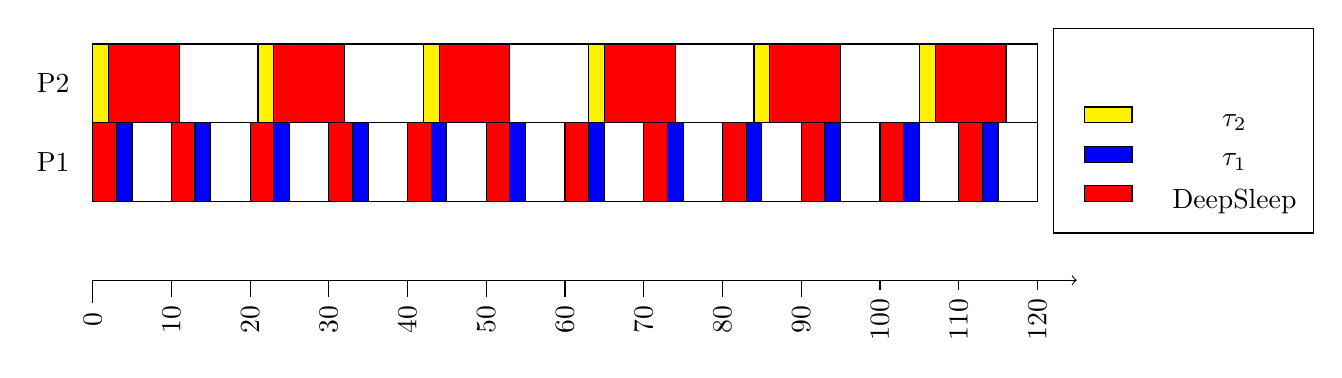
\begin{tikzpicture}
\node at (-0.5,0.5) {P1};
\node at (-0.5,1.5) {P2};
%P1
\draw[fill=white] (0.0,0) rectangle (12,1) ;

\draw[fill=red] (0.0,0) rectangle (0.3,1) ;
\draw[fill=blue] (0.3,0) rectangle (0.5,1) ;

\draw[fill=red] (1.0,0) rectangle (1.3,1) ;
\draw[fill=blue] (1.3,0) rectangle (1.5,1) ;

\draw[fill=red] (2.0,0) rectangle (2.3,1) ;
\draw[fill=blue] (2.3,0) rectangle (2.5,1) ;

\draw[fill=red] (3.0,0) rectangle (3.3,1) ;
\draw[fill=blue] (3.3,0) rectangle (3.5,1) ;

\draw[fill=red] (4.0,0) rectangle (4.3,1) ;
\draw[fill=blue] (4.3,0) rectangle (4.5,1) ;

\draw[fill=red] (5.0,0) rectangle (5.3,1) ;
\draw[fill=blue] (5.3,0) rectangle (5.5,1) ;

\draw[fill=red] (6.0,0) rectangle (6.3,1) ;
\draw[fill=blue] (6.3,0) rectangle (6.5,1) ;

\draw[fill=red] (7.0,0) rectangle (7.3,1) ;
\draw[fill=blue] (7.3,0) rectangle (7.5,1) ;

\draw[fill=red] (8.0,0) rectangle (8.3,1) ;
\draw[fill=blue] (8.3,0) rectangle (8.5,1) ;

\draw[fill=red] (9.0,0) rectangle (9.3,1) ;
\draw[fill=blue] (9.3,0) rectangle (9.5,1) ;

\draw[fill=red] (10.0,0) rectangle (10.3,1) ;
\draw[fill=blue] (10.3,0) rectangle (10.5,1) ;

\draw[fill=red] (11.0,0) rectangle (11.3,1) ;
\draw[fill=blue] (11.3,0) rectangle (11.5,1) ;
%P2
\draw[fill=white] (0.0,1) rectangle (12,2) ;

\draw[fill=yellow] (0.0,1) rectangle (0.2,2) ;
\draw[fill=red] (0.2,1) rectangle (1.1,2) ;

\draw[fill=yellow] (2.1,1) rectangle (2.2999999046325685,2) ;
\draw[fill=red] (2.2999999046325685,1) rectangle (3.1999999046325684,2) ;

\draw[fill=yellow] (4.2,1) rectangle (4.399999809265137,2) ;
\draw[fill=red] (4.399999809265137,1) rectangle (5.299999809265136,2) ;

\draw[fill=yellow] (6.2999997,1) rectangle (6.499999713897705,2) ;
\draw[fill=red] (6.499999713897705,1) rectangle (7.399999713897705,2) ;

\draw[fill=yellow] (8.4,1) rectangle (8.599999618530273,2) ;
\draw[fill=red] (8.599999618530273,1) rectangle (9.499999618530273,2) ;

\draw[fill=yellow] (10.5,1) rectangle (10.7,2) ;
\draw[fill=red] (10.7,1) rectangle (11.6,2) ;
%%%%%%%
\draw [->](0,-1) -- coordinate (x axis mid) (12.5,-1);
\draw (0,-1) -- (0,-1.5) node[fill=white,rotate=90] {0};
\draw (1,-1) -- (1,-1.5) node[fill=white,rotate=90] {10};
\draw (2,-1) -- (2,-1.5) node[fill=white,rotate=90] {20};
\draw (3,-1) -- (3,-1.5) node[fill=white,rotate=90] {30};
\draw (4,-1) -- (4,-1.5) node[fill=white,rotate=90] {40};
\draw (5,-1) -- (5,-1.5) node[fill=white,rotate=90] {50};
\draw (6,-1) -- (6,-1.5) node[fill=white,rotate=90] {60};
\draw (7,-1) -- (7,-1.5) node[fill=white,rotate=90] {70};
\draw (8,-1) -- (8,-1.5) node[fill=white,rotate=90] {80};
\draw (9,-1) -- (9,-1.5) node[fill=white,rotate=90] {90};
\draw (10,-1) -- (10,-1.5) node[fill=white,rotate=90] {100};
\draw (11,-1) -- (11,-1.5) node[fill=white,rotate=90] {110};
\draw (12,-1) -- (12,-1.5) node[fill=white,rotate=90] {120};

\draw[fill=white] (12.2,-0.4) rectangle (15.5,2.2) ;
\draw[fill=red] (12.6,0) rectangle (13.2,0.2) ;
\draw (14.5,0) -- (14.5,0) node[fill=white] {DeepSleep};
\draw[fill=blue] (12.6,0.5) rectangle (13.2,0.7) ;
\draw (14.5,0.5) -- (14.5,0.5) node[fill=white] {$\tau_1$};
\draw[fill=yellow] (12.6,1) rectangle (13.2,1.2) ;
\draw (14.5,1) -- (14.5,1) node[fill=white] {$\tau_2$};
\end{tikzpicture}}
\end{center}
\caption{Insertion globale de tâches d'endormissements dans un multiprocesseur} \label{fig:edfmpl}
\end{figure}
\section{insertion globale}
\begin{figure}[!h]
\begin{center}
\resizebox{15cm}{4cm}{
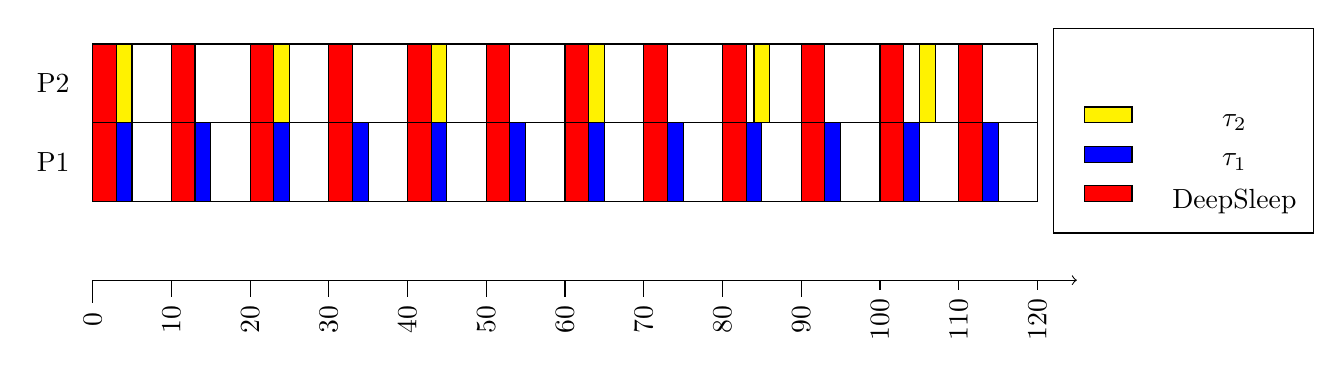
\begin{tikzpicture}
\node at (-0.5,0.5) {P1};
\node at (-0.5,1.5) {P2};
%P1
\draw[fill=white] (0.0,0) rectangle (12,1) ;

\draw[fill=red] (0.0,0) rectangle (0.3,1) ;
\draw[fill=blue] (0.3,0) rectangle (0.5,1) ;

\draw[fill=red] (1.0,0) rectangle (1.3,1) ;
\draw[fill=blue] (1.3,0) rectangle (1.5,1) ;

\draw[fill=red] (2.0,0) rectangle (2.3,1) ;
\draw[fill=blue] (2.3,0) rectangle (2.5,1) ;

\draw[fill=red] (3.0,0) rectangle (3.3,1) ;
\draw[fill=blue] (3.3,0) rectangle (3.5,1) ;

\draw[fill=red] (4.0,0) rectangle (4.3,1) ;
\draw[fill=blue] (4.3,0) rectangle (4.5,1) ;

\draw[fill=red] (5.0,0) rectangle (5.3,1) ;
\draw[fill=blue] (5.3,0) rectangle (5.5,1) ;

\draw[fill=red] (6.0,0) rectangle (6.3,1) ;
\draw[fill=blue] (6.3,0) rectangle (6.5,1) ;

\draw[fill=red] (7.0,0) rectangle (7.3,1) ;
\draw[fill=blue] (7.3,0) rectangle (7.5,1) ;

\draw[fill=red] (8.0,0) rectangle (8.3,1) ;
\draw[fill=blue] (8.3,0) rectangle (8.5,1) ;

\draw[fill=red] (9.0,0) rectangle (9.3,1) ;
\draw[fill=blue] (9.3,0) rectangle (9.5,1) ;

\draw[fill=red] (10.0,0) rectangle (10.3,1) ;
\draw[fill=blue] (10.3,0) rectangle (10.5,1) ;

\draw[fill=red] (11.0,0) rectangle (11.3,1) ;
\draw[fill=blue] (11.3,0) rectangle (11.5,1) ;
%P2
\draw[fill=white] (0.0,1) rectangle (12,2) ;

\draw[fill=red] (0.0,1) rectangle (0.3,2) ;
\draw[fill=red] (1.0,1) rectangle (1.3,2) ;
\draw[fill=red] (2.0,1) rectangle (2.3,2) ;
\draw[fill=red] (3.0,1) rectangle (3.3,2) ;
\draw[fill=red] (4.0,1) rectangle (4.3,2) ;
\draw[fill=red] (5.0,1) rectangle (5.3,2) ;
\draw[fill=red] (6.0,1) rectangle (6.3,2) ;
\draw[fill=red] (7.0,1) rectangle (7.3,2) ;
\draw[fill=red] (8.0,1) rectangle (8.3,2) ;
\draw[fill=red] (9.0,1) rectangle (9.3,2) ;
\draw[fill=red] (10.0,1) rectangle (10.3,2) ;
\draw[fill=red] (11.0,1) rectangle (11.3,2) ;

\draw[fill=yellow] (0.3,1) rectangle (0.5,2) ;
\draw[fill=yellow] (2.3,1) rectangle (2.5,2) ;
\draw[fill=yellow] (4.3,1) rectangle (4.5,2) ;
\draw[fill=yellow] (6.3,1) rectangle (6.5,2) ;
\draw[fill=yellow] (8.4,1) rectangle (8.6,2) ;
\draw[fill=yellow] (10.5,1) rectangle (10.7,2) ;
%%%%%%%
\draw [->](0,-1) -- coordinate (x axis mid) (12.5,-1);
\draw (0,-1) -- (0,-1.5) node[fill=white,rotate=90] {0};
\draw (1,-1) -- (1,-1.5) node[fill=white,rotate=90] {10};
\draw (2,-1) -- (2,-1.5) node[fill=white,rotate=90] {20};
\draw (3,-1) -- (3,-1.5) node[fill=white,rotate=90] {30};
\draw (4,-1) -- (4,-1.5) node[fill=white,rotate=90] {40};
\draw (5,-1) -- (5,-1.5) node[fill=white,rotate=90] {50};
\draw (6,-1) -- (6,-1.5) node[fill=white,rotate=90] {60};
\draw (7,-1) -- (7,-1.5) node[fill=white,rotate=90] {70};
\draw (8,-1) -- (8,-1.5) node[fill=white,rotate=90] {80};
\draw (9,-1) -- (9,-1.5) node[fill=white,rotate=90] {90};
\draw (10,-1) -- (10,-1.5) node[fill=white,rotate=90] {100};
\draw (11,-1) -- (11,-1.5) node[fill=white,rotate=90] {110};
\draw (12,-1) -- (12,-1.5) node[fill=white,rotate=90] {120};

\draw[fill=white] (12.2,-0.4) rectangle (15.5,2.2) ;
\draw[fill=red] (12.6,0) rectangle (13.2,0.2) ;
\draw (14.5,0) -- (14.5,0) node[fill=white] {DeepSleep};
\draw[fill=blue] (12.6,0.5) rectangle (13.2,0.7) ;
\draw (14.5,0.5) -- (14.5,0.5) node[fill=white] {$\tau_1$};
\draw[fill=yellow] (12.6,1) rectangle (13.2,1.2) ;
\draw (14.5,1) -- (14.5,1) node[fill=white] {$\tau_2$};
\end{tikzpicture}}
\end{center}
\caption{} \label{fig:edfmpg}
\end{figure}

\chapter{Expérimentations}
\section{La génération des taches}
\subsection{Cas monoprocesseur}
\subsubsection{Algorithmes UUnifast}
L’algorithme UUnifast [22] est un algorithme mis au point pour la génération de taux d’utilisation
sur monoprocesseur. Il génère une distribution uniforme de n taux d’utilisation non biaisés
à partir du nombre de tâches n de l’ensemble et du taux d’utilisation processeur total souhaité U.
UUnifast est un algorithme efficace de complexité O(n). Nous rappelons qu’un ensemble au taux
d’utilisation supérieur à 1 est trivialement non ordonnançable puisque l’utilisation processeur
dépasse alors le temps maximal disponible.
\subsubsection{Génération des périodes}
Lors de la génération de tâches, le choix des périodes est un élément sensible pour les tests
d’ordonnançabilité. En effet, certains de ces tests basent leur analyse sur un intervalle de faisabilité.
La longueur de cet intervalle dépend du plus petit commun multiple des périodes (ppcm)
appelée l’hyper-période. Si les périodes sont grandes, premières entre elles, l’hyperpériode
explose. Le défi consiste donc à générer des périodes aléatoirement tout en limitant
la taille de l’hyper-période et c’est l’objet de la méthode de Goossens et Macq \cite{Goossens01}. 
\subsubsection{Génération des échéances}
Similairement à Goossens et Macq dans \cite{Goossens01}, nous generons les échéances des taches generées. Nous déterminons
aléatoirement l’échéance dans un intervalle [$0.75 \times T_i$, $T_i$].
En résumé, $Di = \lbrace T_i \times C_i) \times aleatoire(0.75 \times T_i, T_i)\rbrace + C_i$ avec
aleatoire(dmin, dmax) retourne un nombre réel pseudo-aléatoire uniformément distribué sur l’intervalle [dmin, dmax] et où la fonction arrondi(x) retourne l’entier
le plus proche de x.
\subsection{Cas multiprocesseur}
\subsubsection{Algorithme UUnifast-Discard}
La méthode UUnifast présentée dans le cas monoprocesseur n’est pas utilisée en contexte
multiprocesseur, lorsque le taux d’utilisation du processeur U peut dépasser 1. En effet, lorsque
que le taux d’utilisation total dépasse 1, UUnifast présente le risque de générer des taux d’utilisation
par tâche supérieurs à 1. Tâche qu’il n’est alors possible d’ordonnancer sur aucun processeur.
Pour y remédier, Davis et Burns \cite{DB11} ont proposé une extension appelée UUnifast-Discard. Elle
consiste simplement à employer UUnifast avec U supérieur à 1 et à rejeter les ensembles pour
lesquelles au moins un taux d’utilisation par tâche est supérieur à 1. Son implantation est simple
mais cette méthode a l’inconvénient d’être particulièrement inefficace lorsque U approche $\frac{n}{2}$ \cite{Emb10}.
\section{La simulation}
\section{Discussions}